%% This is an example first chapter.  You should put chapter/appendix that you
%% write into a separate file, and add a line \include{yourfilename} to
%% main.tex, where `yourfilename.tex' is the name of the chapter/appendix file.
%% You can process specific files by typing their names in at the 
%% \files=
%% prompt when you run the file main.tex through LaTeX.
\chapter{Introduction}
\section{Motivation}
Large organizations increasingly use virtualization to consolidate server
applications in data centers, reduce operating costs, simplify administrative
tasks and improve performance scalability. As a key 
enabling technology behind {\em Cloud Computing}, virtualization
is shaping how computers will be used in the future.

An important reason for the success of server virtualization 
is that it resolves the tension between typically conflicting
goals of high isolation and effective resource utilization.
Ideally, organizations would assign dedicated
machines for individual server applications
to isolate them. 
However, this approach is inefficient
because each application tends to utilize only a modest fraction of 
the underlying hardware.
With the development of virtualization technology, applications
can be assigned dedicated virtual machines (VMs),
while many such VMs can be hosted on the same physical
host for high resource utilization.

\begin{figure}[p]
  \centering
  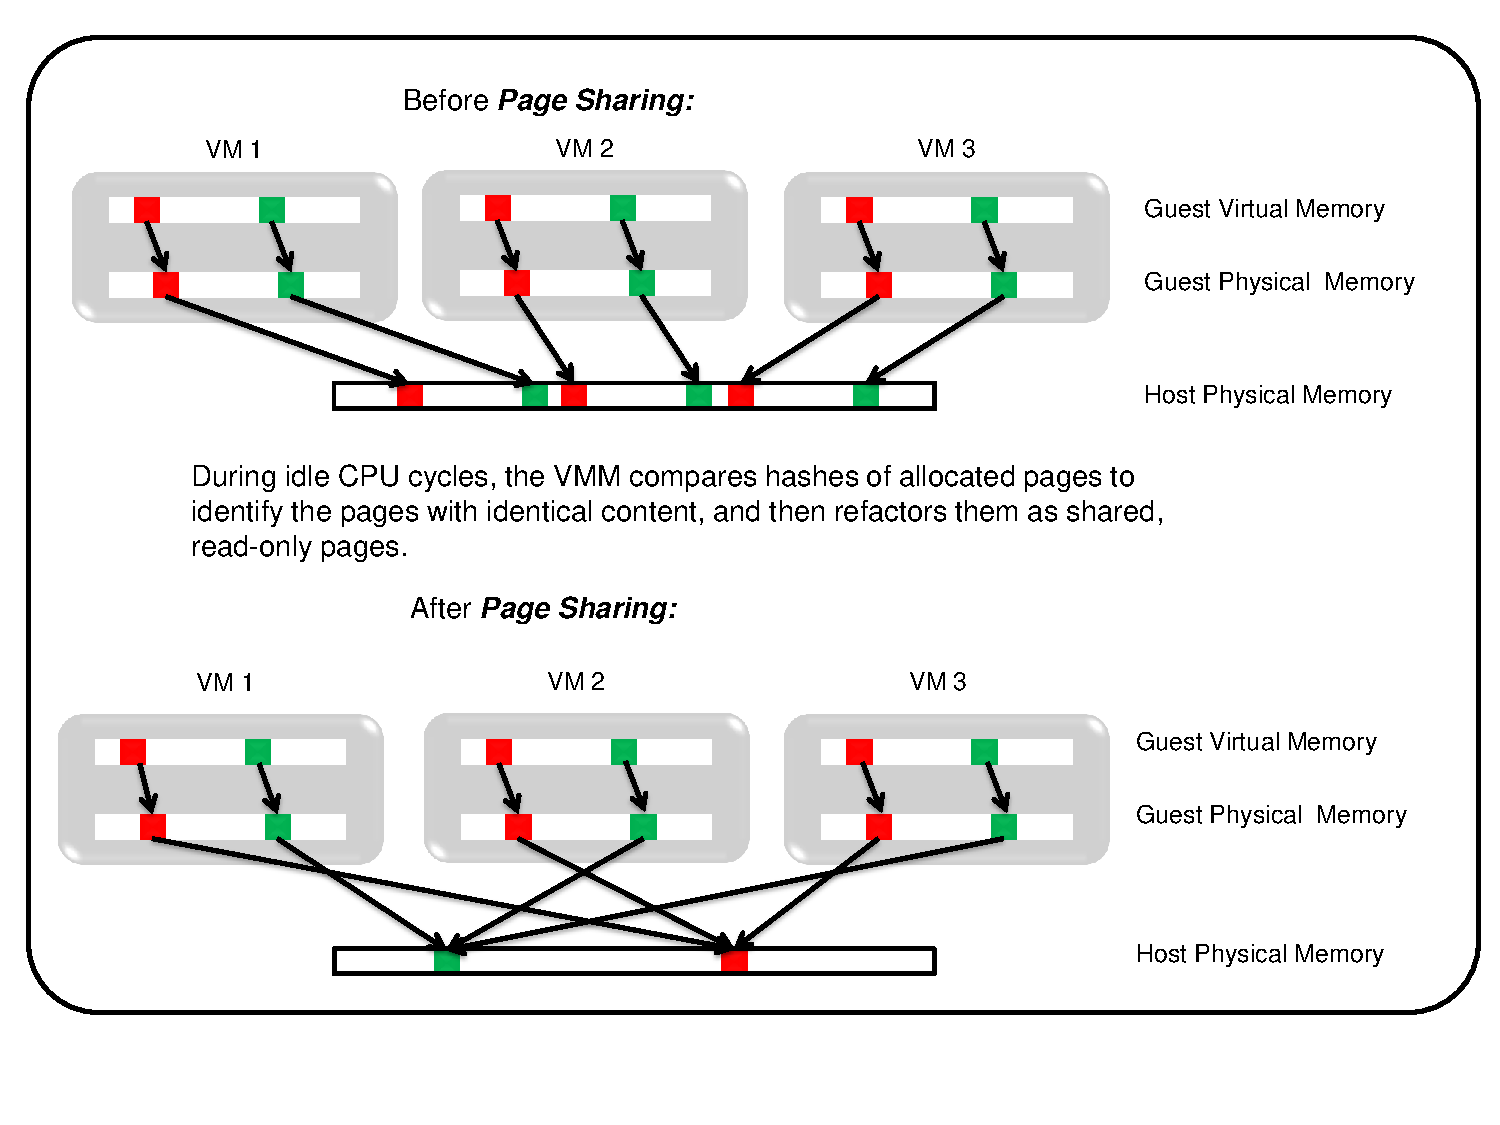
\includegraphics[scale=0.55, trim=1cm 0cm 2cm 0cm]{pagesharing.pdf}  
  \caption[{\em Transparent Page Sharing}]%
          {{\em Transparent Page Sharing}}
          \label{pagesharing}
  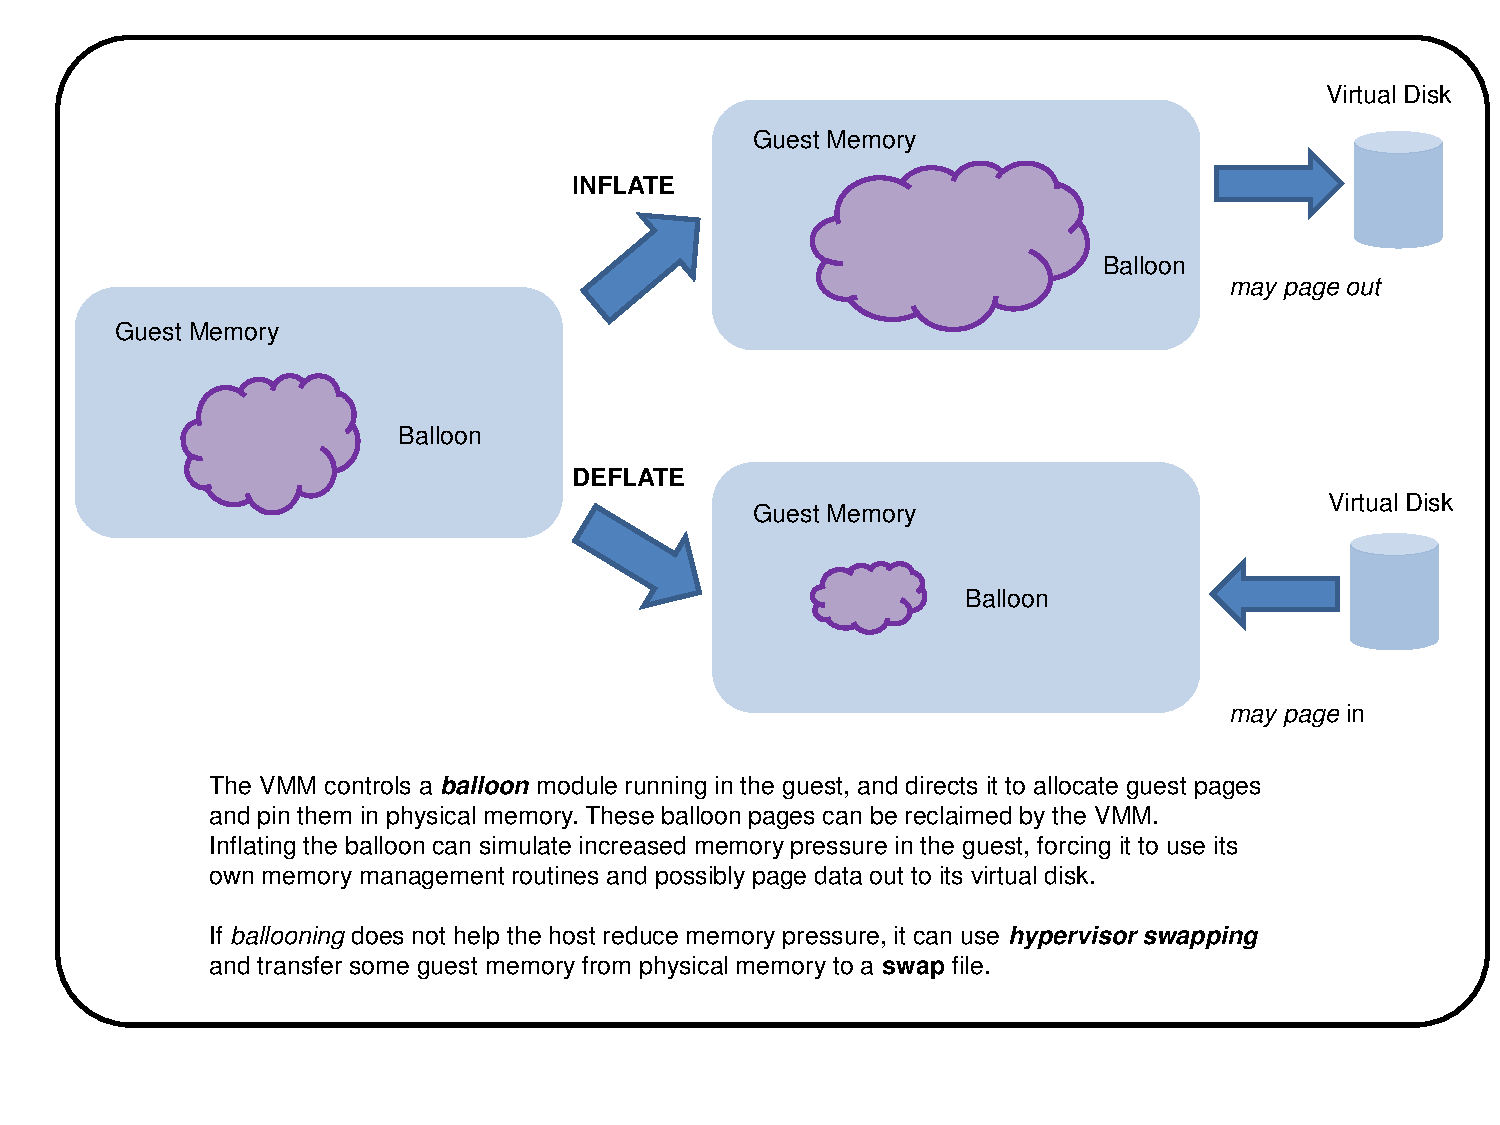
\includegraphics[scale=0.58, trim=1cm 0cm 1cm 0cm]{balloon.pdf}   
  \caption[{\em Ballooning} and {\em Hypervisor Swapping}]%
          {{\em Ballooning} and {\em Hypervisor Swapping}}
          \label{balloon}
\end{figure}


The ability to host many VMs
on the same physical machine is so important to the success
of server virtualization that many companies 
aggressively try to increase {\em VM density per host} by
designing hypervisors for scalability.
For instance, {\em transparent page sharing}, {\em ballooning}
and {\em hypervisor swapping} (see Figures \ref{pagesharing} and \ref{balloon})
allow a host to use {\em memory overcommit} i.e. run VMs with
combined memory requirements
that exceed the total underlying physical memory
available \cite{waldspurger2002memory}. 

Apart from improvements in virtualization technology, two additional trends 
are expected to boost the attainable VM density per host in the future:
\begin{itemize}
\item improvements in hardware available i.e. hosts with
more avalaible memory and processor cores \cite{hansen2010lithium},
and 
\item the anticipated use of Virtual Desktop Infrastructures (VDIs) \cite{vmwarevdi}.
\end{itemize}

In a Virtual Desktop Infrastructure (or a VDI), user {\em desktops} are hosted in
VMs that reside in a data center. 
Users -- typically company employees -- access their virtual desktops via a remote display protocol. 
VDIs provide simplicity in administration and management: applications on 
these VMs can be centrally added, deleted, upgraded and patched. 
Organizations are increasingly investing in VDIs to reap the same benefits
that are offered by server virtualization.

VDI deployments promise even higher VM density per
host than those achieved via server virtualization
because desktop virtual machines typically require
considerably less resources than server virtual machines.
Because of VDIs, hundreds or thousands of identical VMs already are -- or soon
will be -- hosted on individual hosts within data centers.
This is possible because of the low steady-state CPU
usage of a single virtual desktop and the aggressive
use of memory overcommit.

While the {\em steady-state} behavior of desktop VMs
allows many of them to be hosted on a single machine,
correlated spikes in the CPU/memory usage of many VMs can suddenly 
cripple host machines. For instance, a \emph{boot storm} \cite{hansen2010lithium, 
liao2011vmstore, meng2010tide, rajan2010vdc, vaghani2010virtual}
can occur after some software is installed or updated, requiring hundreds 
or thousands of identical VMs to reboot at the same time.
Boot storms can be particularly frequent in VDIs because users typically show up to
work at roughly the same time in the morning each day. 
Concurrently booting VMs create unusually high I/O traffic,
generate numerous disk and memory allocation requests,
and can saturate the host CPU. 
Without any idle CPU cycles, the host cannot use transparent page sharing,
which also increases memory pressure.
Many data centers thus simply cannot sustain a high VM density 
per host during boot storms without incurring
prohibitively high boot latencies that result
from saturated CPUs and stressed hardware.

To mitigate boot storms, data centers usually
boot VMs in a staggered fashion, or invest in specialized,
expensive and/or extra-provisioned hardware \cite{highperfnas, liao2011vmstore}.
Anecdotal evidence suggests that VDI users sometimes leave their desktop computers running
overnight to prevent morning boot storms; this practice
represents an unnecessary addition to already exorbitant
data center energy bills \cite{qureshi2009bills}. 
While data deduplication \cite{clements2009deduplication}
can mitigate the stress on the storage layer in
a boot storm, lowered memory latency can in turn overwhelm the CPU, 
fibre channel, bus infrastructure or controller resources 
and simply turn them into bottlenecks instead \cite{netappstorm}. 

With the spread of virtualization, we believe that it is important to address the
boot storm problem in a way that does not skirt around the issue
and enables data centers to sustain a high VM density per host even
during boot storms. {\em Page sharing} is effective
in general because many VMs access similar pages during execution.
Inspired by this idea, we pose a few simple questions: 
if many identical VMs concurrently boot up on the same host,
do they execute the same set of instructions? Even if there are
some differences in the instructions executed, are they caused by
controllable sources of nondeterminism? Ultimately, if there is a way
to ensure that concurrently booting VMs execute mostly the same set of instructions,
 one way to retain a high VM density 
per host in boot storms may be remarkable simple in essence:
the hypervisor could identify the overlap in the instruction streams of 
the VMs to avoid repetitive execution and reduce
CPU pressure. Just like {\em page sharing} (i.e. eliminating page
duplication) allows hosts to use memory resources in a scalable fashion in
the steady-state, perhaps {\em silhouette exection} (i.e. eliminating
instruction duplication) will allow hosts to use CPUs in a more scalable fashion during boot storms.

\section{Goal of Thesis}
This thesis aims to address the following questions:

\begin{enumerate}

\item When identical VMs boot up at the same time, how similar
are the sets of instructions executed? What is the statistical
profile of any differences in the executed instructions?

\item What are the source(s) of any differences in
the multiple instruction streams of concurrently booting VMs?

\item Are there ways to minimize the execution differences (or {\em nondeterminism})
across multiple booting VMs?

\end{enumerate}

The answers to these questions are clearly crucial in determining
the feasibility of \emph{silhouette execution} as a possible solution
to the boot storm problem. 

\section{Contributions}
For this work, we used Pin \cite{luk2005pin},
a dynamic instrumentation framework,
to study user-mode instruction streams from 
a few Linux services at boot-time. 
Specifically, we:
\begin {enumerate}
\item quantify nondeterminism in Linux services, and show that it is
  bursty and rare;
\item document the sources of nondeterminism in Linux services -- both obvious and obscure;
\item mathematically model the effectiveness
  of {\em silhouette execution} in user-space. Using simulations, we provide conservative estimates for the possible change in the number of instructions
  executed in user-space by a host CPU when many VMs boot up with silhouette execution than without it;
\item propose several simple techniques (e.g. {\em I/O} and {\em signal alignment}, {\em process ID virtualization})
  to reduce the overhead in silhouette execution from controllable nondeterminism.
\end {enumerate}

Through our simple models, we estimate that silhouette execution {\em increases} the number
of instructions executed in user-space by 13\% for 100 VMs and 6\% for 1000 VMs and 
over the status-quo. However, after we use our proposed strategies to reduce synthetic execution differences
between VMs, silhouette execution {\em reduces} the number of instructions executed
by a factor of $8\times$ for 100 VMs and $19\times$ for 1000 VMs over the status-quo 
in our simulations.

Strategies to achieve deterministic execution have been proposed at the operating system layer \cite{bergan2010dos} before,
but they require modifications to Linux. Nondeterminism in multi-threaded programs 
can be reduced via record-and-replay approaches \cite{patil2010pinplay} or deterministic logical clocks \cite{marek2011scaling}. 
Our study has different goals from from both approaches: we wish to avoid changing existing 
software (to ease adoption); we also wish to make several distinct -- and potentially different -- executions \emph{overlap} as much as possible, 
rather than replay one execution over and over.
In our case, we do not know \emph{a priori} whether two executions 
will behave identically or not. That the behavior of system calls or signals in Linux can lead to different results or side-effects across
multiple executions of an application is well known: what is not documented is the application \emph{context} in
which these sources of nondeterminism originate, which we had to investigate to identify
ways to improve silhouette execution. \newline

\noindent To the best of our knowledge,
\begin {itemize}
\item this is the first attempt to study the statistical profile and context of execution differences
  across multiple instances of Linux services during boot;
\item exploiting overlap in instruction streams to reduce CPU pressure (i.e. {\em silhouette execution}) is a novel 
  design idea, and we are the first to introduce designs for it and mathematically model its effectiveness.
\end {itemize}

\noindent Ultimately, we hope that our work will be the foundation for a real-world implementation of {\em silhouette execution},
and in turn, a long-term solution to the VM boot storm problem. 

\section{Importance of Deterministic Execution}
Our study of nondeterminism was driven by a specific application,
deterministic execution is desirable in a variety of scenarios.
The motivations for deterministic multhreading listed in
\cite{marek2011scaling, patil2010pinplay} apply to our work as well. \newline

\noindent {\bf Silhouette Execution} \newline 
Controlling nondeterminism in the execution of concurrently
booting VMs greatly improves silhouette execution, because the hypervisor
can hypothetically exploit the greater overlap or redundancy
across distinct instruction streams to use the CPU
in a scalable way during boot storms. \newline

\noindent {\bf Transparent Page Sharing} \newline
Idle CPU cycles in the hypervisor are necessary for transparent page sharing
to be effective in the background. Thus, reducing CPU 
pressure through determinism and silhouette execution clearly facilitates
transparent page sharing during boot storms.
More generally, removing synthetic differences due to controllable nondeterminism in the execution
of concurrently running VMs can improve transparent page sharing
as well, because the contents of data accessed/written are more likey
to be similar when minor differences due to e.g. process IDs,
timestamps or execution statistics are eliminated. \newline

\noindent {\bf Mainstream Computing, Security and Performance} \newline
If distinct executions of the same program can be
expected to execute similar sets of instructions, then
significant deviations can be used to detect security
attacks. Runtime detection of security attacks through the
identification of anomalous executions is the focus of \emph{mainstream computing} \cite{stephenson2010mainstream},
and deterministic execution obviously helps in reducing false
positives. 
Anomalous executions can also be flagged for performance
debugging. \newline

\noindent {\bf Testing}  \newline
Deterministic execution in general facilitates testing,
because outputs and internal state can be checked at 
certain points with respect to expected values. 
Sometimes, a particularly strong 
test case may be necessary for safety-critical 
systems: a program 
must execute the exact same instructions 
across different executions (for the same inputs). \newline 

\noindent {\bf Debugging} \newline 
Erroneous behavior can be more easily reproduced
via determininstic execution, which
helps with debugging. Deterministic
execution has much lower storage overhead
than traditional record-and-replay approaches. 

\section{Thesis Organization} 
In what follows, Chapter \ref{ch:boot} presents an overview of
the Linux boot process, along with the dynamic instrumentation
techniques we used to profile nondeterminism in Linux services.
Chapter \ref{ch:src} presents a summary of the sources of nondeterminism
discovered in this work.
Chapter \ref{ch:sil} introduces {\em silhouette execution},
outlines the simple simulations we used to model
and evaluate its feasibility in user-space,
and presents simple design strategies to 
improve its effectiveness.
Finally, Chapter \ref{ch:conc} concludes this thesis and discusses future work.
